\section{Relativistic Kinematics}
The conversion from one reference frame to another is done by the linear Lorentz transformation. The Lorentz transformation is given by \cref{eq: Lorentz_transformation} where $β = v / c$ and $γ 1 / \sqrt{1 - β^2}$. 
\begin{equation}\label{eq: Lorentz_transformation}
    \begin{pmatrix*}[r]
     ct \\
     x \\
     y \\
     z 
    \end{pmatrix*}' = 
    \begin{pmatrix*}[r]
     γ & 0 & 0 & -γβ \\
     0 & 1 & 0 & 0 \\
     0 & 0 & 1 & 0 \\
     -γβ & 0 & 0 & γ 
    \end{pmatrix*} 
    \begin{pmatrix*}[r]
     ct \\
     x \\
     y \\
     z 
    \end{pmatrix*} \ , \ 
    \begin{pmatrix*}[r]
     E / c \\
     p_x \\
     p_y \\
     p_z 
    \end{pmatrix*}' = 
    \begin{pmatrix*}[r]
     γ & 0 & 0 & -γβ \\
     0 & 1 & 0 & 0 \\
     0 & 0 & 1 & 0 \\
     -γβ & 0 & 0 & γ
    \end{pmatrix*}
    \begin{pmatrix*}[r]
     E / c \\
     p_x \\
     p_y \\
     p_z
    \end{pmatrix*}
\end{equation}
\paragraph{Example:}
For a particle at rest in coordinate system $s$, we have $\vec{p} = 0$ and $E = mc^2$. From here we can derive the energy and momentum in the $s'$ system.
\begin{equation}
  p_{z}' = - \frac{γβE}{c} = -mγβc = -mvγ
\end{equation}
\begin{equation}
  E' / c = γE / c = ymc → E' = γmc^2
\end{equation}
In this case we have $p'_{\perp} = p_{\perp}$, as the transformation is in the z-direction.

\subsection{Four-Vectors}
\begin{align}
    \vec{A} &= (A_0, a_x, a_y, a_z) \\
    \vec{B} &= (B_0, b_x, b_y, b_z)
\end{align}
\subsubsection{Dot product}
\begin{equation}
  \vec{A} ⋅ \vec{B} = A_0B_0 - a_xb_x - a_yb_y - a_zb_z ) \vec{A}^{T} η \vec{B}
\end{equation}
\begin{equation}
  η = 
    \begin{pmatrix*}[r]
    1 & 0 & 0 & 0 \\
    0 & -1 & 0 & 0 \\
    0 & 0 & -1 & 0 \\
    0 & 0 & 0 & -1
    \end{pmatrix*}
\end{equation}
\subsubsection{Dot product in different reference frames}
\begin{equation}
    \vec{A}' ⋅ \vec{B}' = 
    \begin{pmatrix*}[r]
    A_0 \\
    a_x \\
    a_y \\
    a_z
    \end{pmatrix*}^{T} 
    \begin{pmatrix*}[r]
    γ & 0 & 0 & -γβ \\
    0 & 1 & 0 & 0 \\
    0 & 0 & 1 & 0 \\
    -γβ & 0 & 0 & γ
    \end{pmatrix*} 
    \begin{pmatrix*}[r]
    1 & 0 & 0 & 0 \\
    0 & -1 & 0 & 0 \\
    0 & 0 & -1 & 0 \\
    0 & 0 & 0 & -1
    \end{pmatrix*}
    \begin{pmatrix*}[r]
    γ & 0 & 0 & -γβ \\
    0 & 1 & 0 & 0 \\
    0 & 0 & 1 & 0 \\
    -γβ & 0 & 0 & γ
    \end{pmatrix*}
    \begin{pmatrix*}[r]
    B_0 \\
    b_x \\
    b_y \\
    b_z \\
    \end{pmatrix*}
\end{equation}
Using the fact that $(ab)^{T} = b^{T} a^{T}$ we get:
\begin{equation}
    \vec{A}' ⋅ \vec{B}' = 
    \begin{pmatrix*}[r]
    A_0 \\
    a_x \\
    a_y \\
    a_z
    \end{pmatrix*}^{T}
    \begin{pmatrix*}[r]
    1 & 0 & 0 & 0 \\
    0 & -1 & 0 & 0 \\
    0 & 0 & -1 & 0 \\
    0 & 0 & 0 & -1
    \end{pmatrix*}
    \begin{pmatrix*}[r]
    B_0 \\
    b_x \\
    b_y \\
    b_z
    \end{pmatrix*} = \vec{A} ⋅ \vec{B}
\end{equation}
\subsubsection{Attributes Summary}
Consider the following attributes of the dot product of two four-vectors $\vec{A} = (ct,\vec{x})$ and $\vec{B} = (E / c , \vec{p})$. 
\begin{itemize}
    \item The dot product is invariant under Lorentz transformations. This means that the dot product is the same in all reference frames.
    \item $\vec{A}^2 = \vec{A} ⋅ \vec{A} = c^2t^2 - \left|\vec{x}\right|^2 = $ constant. 
    \item $\vec{B}^2 = E^2 / c^2 - \left|\vec{p}\right|^2 = $ constant. We define the invariant mass as mass in the rest frame. 
    \begin{equation}
      (Wc^2)^2 = E^2 - \left|\vec{p}\right|^2c^2
    \end{equation}
    If $\vec{p} = 0$ then $(Wc^2)^2 = E^2 = m^2c^{4}$, which makes $m = W$, the rest mass. 
    \item The invariant mass for a collation of particles is defined as the sum of the invariant masses of the particles.
    \begin{equation}
      (Wc^2)^ ≡ \left(∑_{i}^{} E_i\right)^2 - \left(∑_{i}^{} \left|\vec{p}_i\right|\right)^2c^2
    \end{equation}
    This allows us to measure the mass in any frame we find convenient. This allowed us to detect the Higgs boson, by looking at the invariant mass of the decay products which were photons. 
\end{itemize}

\subsection{Four-Momentum Transfer}
\begin{equation}
  Q^2 ≡ - \left(E - E'\right)^2 - \left(c \vec{p} - c \vec{p}'\right)^2 = - c^2 \left(\vec{P}_i - \vec{P}_f\right)^2
\end{equation}
Since $Q^2$ is dependant on the Lorenz invariant four-vectors, it is also Lorenz invariant. The probability amplitude for the Yukawa potential is therefore: 
\begin{equation}
  \mathcal{M} (Q^2) = \frac{-g^2 ℏ^2}{Q^2 + m^2 c^2}
\end{equation}
which is also Lorenz invariant.

\subsection{Invariant Mass of Virtual Photon}
Consider the following reaction:
\begin{equation}    
  e^{+} e^{-} → γ^{*} / Z^{*} → f \bar{f}
\end{equation}
We have a symmetric collider which $E_{b} → ← E_{b}$. The momentum of the virtual photon is 0. 
\begin{equation}
  \vec{p}_{γ}^{*} = 0 → Wc^2 = 2E_{b}
\end{equation}
We can then find the center mass energy:
\begin{equation}
  \sqrt{s} = Wc^2 = E_{\text{cm}} = 2E_{b}
\end{equation}

\subsubsection{Fixed-Target Experiment}
Consider a particle collision between a beam $b$, and a target $t$ at rest. How do we find the center mass energy?
\begin{equation}
  E_{b}^2 = m^2_{b}c^{4} + p^2_{b}c^{2} \quad , \quad  E_t = m_{t}c^{2}
\end{equation}
\begin{equation}
  (Wc^2)^2 = \left(∑_{i}^{} E_i\right)^2 - \left(∑_{i}^{} \left|\vec{p}_i\right|\right)^2c^2 = \left(E_{b} + m_tc^2\right)^2 - \left(\vec{p}_{b}c\right)^2
\end{equation}
If we let $c = 1$, we find $W$. 
\begin{equation}
  W = E_{\text{cm}} = \sqrt{m_{b}^2 + m_{t}^2 + 2E_{b}m_{t}}
\end{equation}
If the momentum is very large, we can neglect the masses of the particles so $E_{\text{cm}} = \sqrt{2m_{t}E_{b}}$. 

\section{Particle Accelerators}
\begin{itemize}
    \item Particles are accelerated by a voltage. This has a 1-1 correspondence with the energy for the electrons. Using a voltage of 1 MeV, we can accelerate electrons to an energy of 1 MeV.
    
\end{itemize}

\subsection{Linear Accelerators}
\begin{itemize}
    \item At high voltages, the field breaks down. Using an alternating current, we can avoid this.
    \item Radio frequency linear accelerators are used to accelerate particles to any energy, as the particle only feels the electric energy in the gaps. This is illustrated in \cref{fig: rad-freq_lin_acc}.
    \begin{figure}[h!]
    \centering
    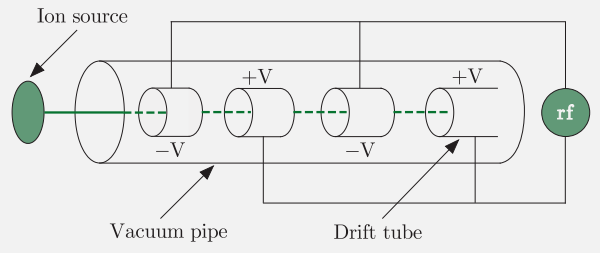
\includegraphics[width = .7\textwidth]{rad-freq_lin_acc.png}
    \caption{Illustration of a radio frequency linear accelerator. The voltages oscillate as the particles moves through the gaps. Only every second tube can be occupied. }
    \label{fig: rad-freq_lin_acc}
    \end{figure}
\end{itemize}

\subsection{Cyclotrons}
\begin{itemize}
    \item Using an oscillating current, the particle will start in the center, and spiral outwards. This is illustrated in \cref{fig: cyclotron}.
    \begin{figure}[h!]
    \centering
    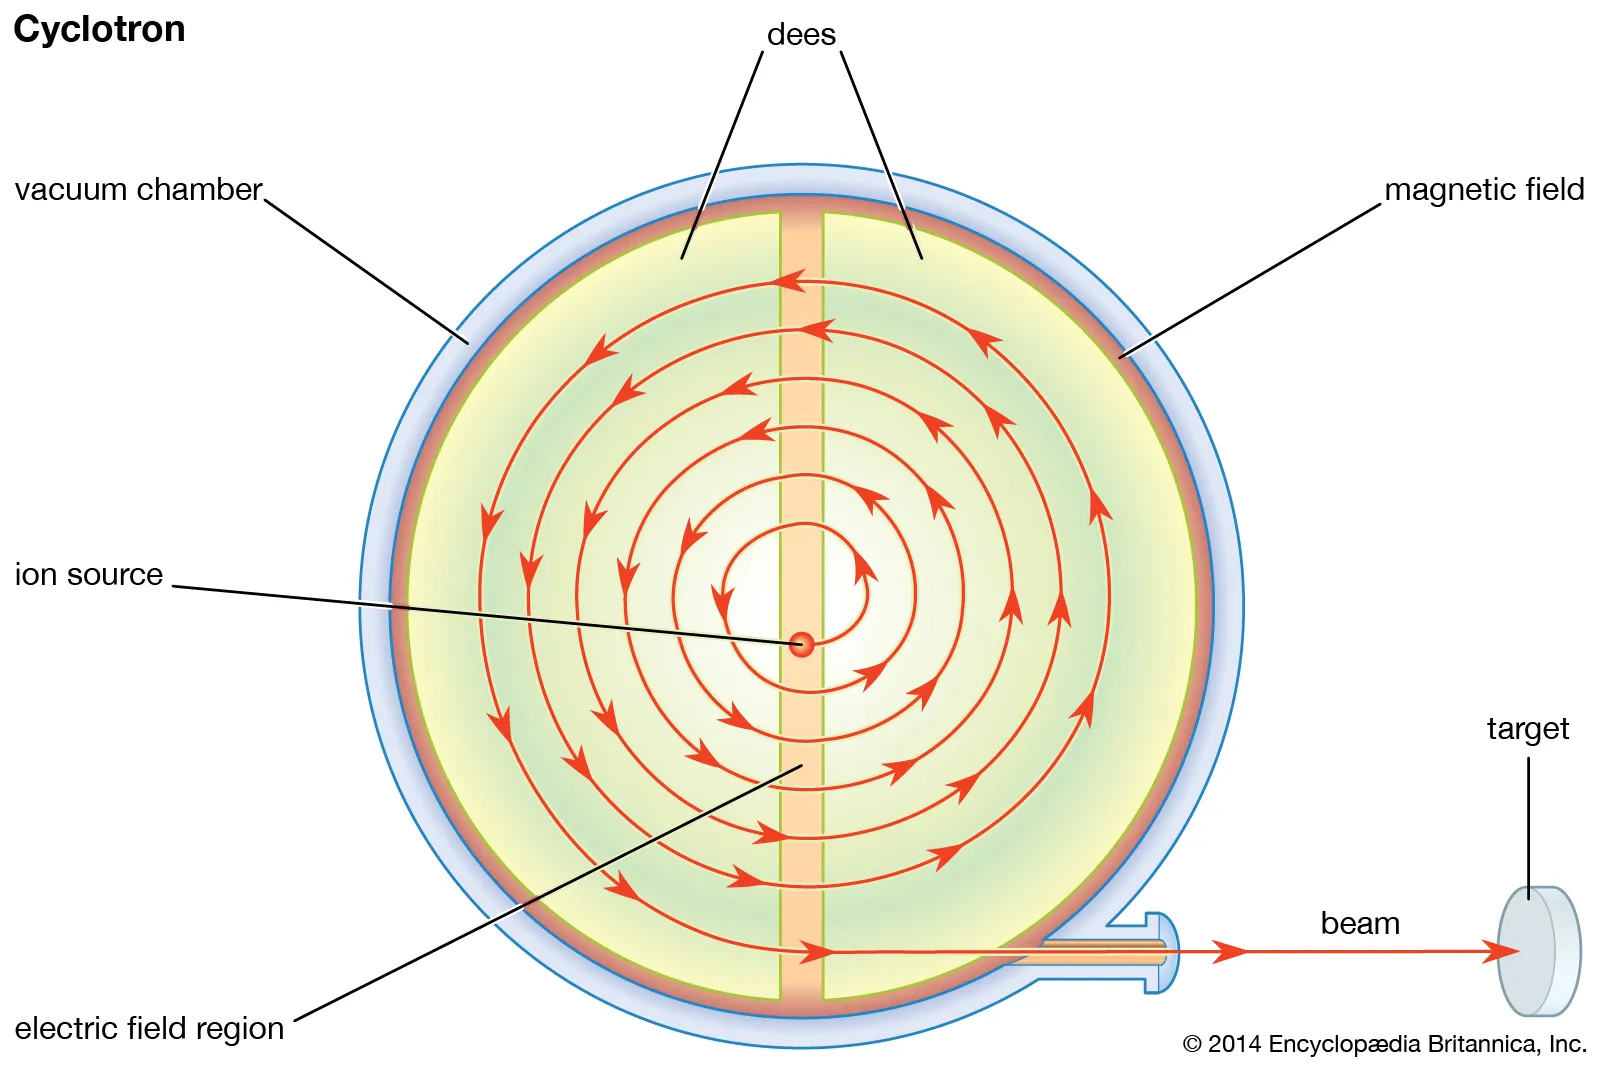
\includegraphics[width = .6\textwidth]{cyclotron.png}
    \caption{Illustration of a cyclotron. }
    \label{fig: cyclotron}
    \end{figure}
\end{itemize}

\subsection{Focusing of Particles}
\begin{itemize}
    \item Magnetic fields are used to focus the beam to a point. 
    \item Quadrupole magnets (4 poles) are often used. They work analogously to a optical lense. 
    \item The ability to focus the beam of some width $σ(s)$ is limited by the focusing properties $β(s)$ (the magnets) and how much each particle deviates from the beam $ε$. 
    \begin{equation}
      σ(s) = \sqrt{εβ(s)}
    \end{equation}
\end{itemize}

\subsection{Characteristics of Accelerators}
\begin{itemize}
    \item \textbf{Particle Type:} Protons, electrons, ions, etc.
    \item \textbf{Center of mass energy:} You need a certain amount of energy to create the different particles. You need $E_{\text{cm}} ≥ mc^2$. The wavelength of the particles is given by $λ = \frac{h}{p}$. You need a probe with an even smaller wavelength. 
    \item \textbf{Luminosity:} $R = \mathcal{L}σ$ where $\mathcal{L} = f n_1n_2 / 4πσ_xσ_y$. This shows the production rate $R$ needed. $n_1$ and $n_2$ are the number of particles, $σ_x$ and $σ_y$ are the transverse sizes of the beams. $f$ is the rate of collisions. 
\end{itemize}

\subsection{Large Hadron Collider (LHC)}
\begin{itemize}
    \item Circumference of 27 km.
    \item Four interaction points where the beams collide.
    \item Eight straight sections of 530m, leading to the IPs (intersection points). 
    \item 1200 superconducting dipole magnets are used to bend the beams.
    \item Can bunch $n = 1e 11$ protons with a collision frequency $f = 40$MHz. These are focused to a width of $σ = 20μ$m at the IP.
\end{itemize}

\subsection{Particle Types}
\begin{itemize}
    \item \textbf{Proton-Proton Colliders:} Initial state is unknown. There is a lot of background noise, which must be filtered.
    \item \textbf{Electron-Positron Colliders:} Initial state is known. The background noise is lower.
\end{itemize}


\subsection{Limitations}
\begin{itemize}
    \item \textbf{Circular proton-proton collider:} The strength of the magnetic fields limits the energy.  
    \item \textbf{Circular electron-positron collider:} The radiation loss makes it hard to reach high energies.
    \item \textbf{Linear electron-positron collider:} The width of the beam is a lot larger, making the luminosity requirements harder to reach.
\end{itemize}
